\documentclass[11pt, oneside]{article} 
\usepackage{geometry}
\geometry{letterpaper} 
\usepackage{graphicx}
	
\usepackage{amssymb}
\usepackage{amsmath}
\usepackage{parskip}
\usepackage{color}
\usepackage{hyperref}

\graphicspath{{/Users/telliott_admin/Dropbox/Tex/png/}}
% \begin{center} 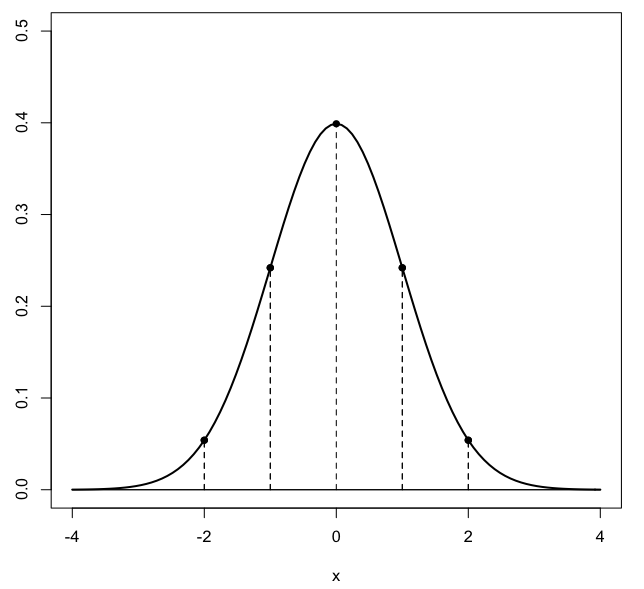
\includegraphics [scale=0.4] {gauss3.png} \end{center}

%break
\title{Polar area}
\date{}

\begin{document}
\maketitle
\Large
Here are some fancy examples of polar curves from \emph{The Calculus Lifesaver}.
\begin{center} 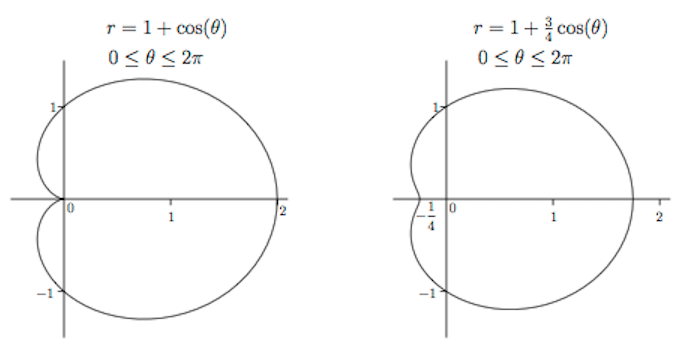
\includegraphics [scale=0.5] {polarex1.png} \end{center}
\begin{center} 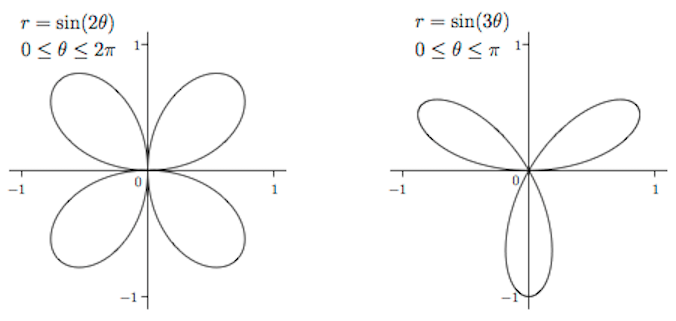
\includegraphics [scale=0.5] {polarex2.png} \end{center}
\begin{center} 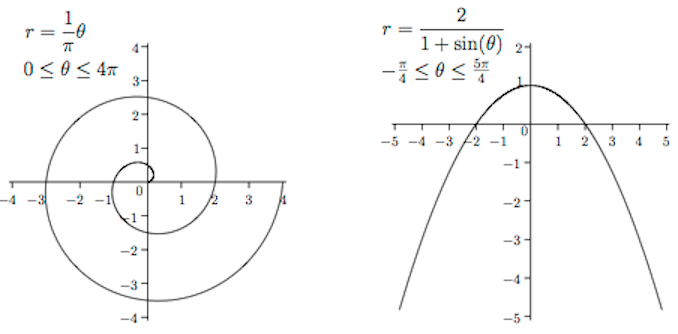
\includegraphics [scale=0.5] {polarex3.png} \end{center}

\subsection*{Integration to find areas}

The idea for (one-dimensional) integration in polar coordinates is that we know $r$ as a function of $\theta$.  For example, we had the circle centered at $(0,3/2)$ given by

\[ r = 3 \sin \theta \]

We imagine dividing up the circle into little triangles, sectors where 

\[ \theta \rightarrow \theta + \Delta \theta \]

The sector is approximately a triangle with side $r$ and base $r \times \Delta \theta$ (the latter is the length of the arc of the circle on its circumference).

The area of each little sector is

\[ \frac{1}{2} r^2 d \theta \]
\subsection*{example}
For this problem:
\[ r = 3 \sin \theta \]

The total area is then
\[ \int_0^{2\pi}  \frac{1}{2} r^2 d \theta \]
\[ = \int_0^{2\pi}  \frac{1}{2} (3 \sin \theta)^2 d \theta \]
\[ = \frac{9}{2} \int_0^{2\pi}  \sin^2 \theta d \theta \]

This looks hard but we've done it before.  One way is to recall that 

\[ [ \ \sin \theta \cos \theta \ ]' = - \sin^2 \theta + \cos^2 \theta \]
\[ =  1 - 2 \sin^2 \theta \]
Integrate
\[ \int [ \ \sin \theta \cos \theta \ ]' \ d \theta = \int (1 - 2 \sin^2 \theta) \ d \theta \]
\[ \sin \theta \cos \theta  = \theta - 2 \int \sin^2 \theta \ d \theta \]
Hence
\[ \int \sin^2 \theta \ d \theta = \frac{1}{2}  (\theta - \sin \theta \cos \theta) \]

So our answer is

\[ = (\frac{9}{2}) \ \frac{1}{2} (x -  \sin \theta \cos \theta) \ \bigg |_0^{2\pi} \]
\[ =  (\frac{9}{2}) \ \frac{1}{2} (2 \pi) \]
\[ = \frac{9\pi}{4} \]

which is correct for a circle with radius $3/2$.
\subsection*{example}
The second example is from \emph{How to ace the rest of calculus}.  We have two circles, both of radius $1$.  The first one is centered at the origin.  We are given the equation of the second in polar coordinates:
\[ r = 2 \cos \theta \]
Plugging in some values for $\theta$: and calculating $r$:
\[ \theta = 0 \rightarrow r = 2 \]
\[ \theta = \frac{\pi}{6} \rightarrow r = \frac{\sqrt{3}}{2} \]
\[ \theta = \frac{\pi}{4} \rightarrow r = \sqrt{2} \]
\[ \theta = \frac{\pi}{3} \rightarrow r = 1 \]
\[ \theta = \frac{\pi}{2} \rightarrow r = 0 \]

We can also convert to $x,y$-coordinates.  Multiply by $r$:
\[ r^2 = 2 r \cos \theta \]
Substituting $r^2 = x^2 + y^2$ and $x = r \cos \theta$:
\[ x^2 + y^2 = 2x \]
Complete the square:
\[ (x^2 - 2x + 1) + y^2 = 1 \]
\[ (x-1)^2 + y^2 = 1 \]
The second circle is centered at $(1,0)$.  Note that for this circle it is \emph{not} true that $x^2 + y^2 = 1$.

Now, the problem given is to calculate the shaded area in the figure.
\begin{center} 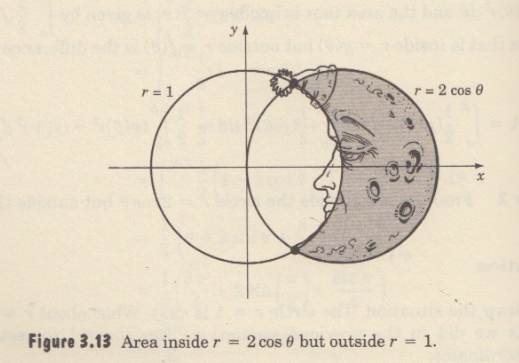
\includegraphics [scale=0.5] {two-circles.png} \end{center}
First, we must find the value of $\theta$ at the points of intersection between the two circles.  We solve the two equations simultaneously:
\[ y^2 = 1 - x^2 \]
\[ (x - 1)^2 + y^2 =  (x - 1)^2 + 1 - x^2 = 1 \]
\[ -2x + 2 = 1 \]
\[ 2x = 1 \]
\[ x = \frac{1}{2} \]
\[ y = \sqrt{1 - x^2} = \pm \frac{\sqrt{3}}{2} \]
\[ \theta = \tan^{-1} \frac{y}{x} = \pm \sqrt{3} \]
Look it up:
\[ \theta = \pm \frac{\pi}{3} \]
or notice that we are on the unit circle so $\cos \theta = x = 1/2$, $\theta = \pm \pi/3$.
That's the hard way.  The easy way is
\[ r = 1 = 2 \cos \theta \]
\[ \theta = \cos^{-1} \frac{1}{2} = \frac{\pi}{3} \]

The area of an arc of the unit circle is the $r^2$ times one-half the arc length in radians.
\[ A = \frac{1}{2} \ \int r^2 \ d \theta \]
We will subtract the area of the inner arc from that covered by the outer one
\[ A = \frac{1}{2} \int_{-\pi/3}^{\pi/3} (2 \cos \theta)^2 - 1 \ d \theta \]
Recall that
\[ \cos 2 \theta = \cos^2 \theta - \sin^2 \theta = \cos^2 \theta - 1 + \cos^2 \theta \]
\[ \cos^2 \theta = \frac{1}{2} (1 + \cos 2 \theta) \]
so
\[ (2 \cos \theta)^2 = 4 \ \frac{1}{2} (1 + \cos 2 \theta) = 2(1 + \cos 2 \theta) \]
\[ A = \frac{1}{2} \int_{-\pi/3}^{\pi/3} (2 \cos \theta)^2 - 1 \ d \theta \]
\[ = \frac{1}{2} \int_{-\pi/3}^{\pi/3} 2 \cos 2 \theta + 1 \ d \theta \]
\[ = \frac{1}{2} \ [ \ \sin 2 \theta + \theta \ ] \ \bigg |_{-\pi/3}^{\pi/3} \]
Since $\sin 2 \pi / 3 = \sqrt{3}/2$:
\[ = \frac{1}{2} (\sqrt{3} + \frac{2 \pi}{3}) = \frac{\sqrt{3}}{2} + \frac{\pi}{3} \]

\end{document}  